

Systems that react to stimuli are all around us. However, many systems don't behave as we want them to. Control theory is a framework that allows engineers to find ways to manipulate these stimuli in order to get these systems to behave as they want them to. Traditionally, the first step to controlling a system is to model the underlying system. If the system is a linear time-invariant (LTI) system, it can be modelled by a transfer function or state space equations. This transfer function or state space model is a parametric representation of the system. When a parametric model of the system is obtained, a controller can be designed for it. 

A model of an LTI system can be obtained by applying a well-designed input to the system and measuring the corresponding output.

Data-driven control is an attempt to skip the modelling part of this process. Instead of going from data to a parametric model to a controller, a controller is found directly from data. This is illustrated in figure \ref{fig:data-driven_vs_tradition}.

One such data-driven approach is model reference control \cite{Data-driven_model_reference_control}. The idea is to define a reference model and to tune a controller such that the closed loop system is as close as possible to the reference model. However, as will be shown in chapter \ref{chapter:model_reference_control}, the name ``data-driven'' can be a bit misleading. In fact, it will be shown that a nonparametric model is hidden in the maths. A nonparametric model differs from a parametric model in the sense that the parametric model tries to describe the data using a relatively small amount of parameters. A nonparametric model still has parameters, but the amount of parameters can be equal to the number of data points. Concretely, applied to LTI systems, a parametric model could be a transfer function where the parameters are the coefficients of the numerator and denominator. A nonparametric model of an LTI system could be the frequency response function at different frequencies.

Chapter \ref{chapter:preliminaries} gives an introduction to nonparametric models of LTI systems. Chapter \ref{chapter:model_reference_control} explains model reference control and shows that there is an underlying nonparametric model in the maths. Chapter \ref{chapter:guaranteed_stability} shows how stability can be guaranteed in model reference control in the absence of a parametric model and in chapter \ref{chapter:real_experiment} model reference control is used to design a controller for a real system.


\begin{figure}
\centering
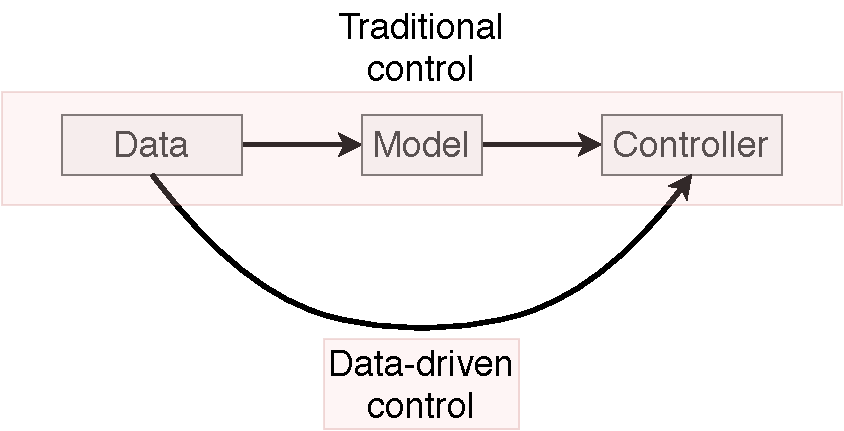
\includegraphics[width = 0.7\textwidth]{figures/data-driven_vs_tradition.pdf}
\caption{Traditional control vs. data-driven control.}
\label{fig:data-driven_vs_tradition}
\end{figure}
